\documentclass[10pt, handout]{beamer}
\usepackage{xmpincl}
\includexmp{license}
\usepackage[T1]{fontenc}
\usepackage[latin1]{inputenc}
\usepackage{ae}
\usepackage[french]{babel}
\usepackage{array, longtable}
\usepackage{tikz}
\usetikzlibrary{arrows,shapes,trees,fit,decorations.pathmorphing,backgrounds}
\usetheme{Antibes}
\setbeamertemplate{navigation symbols}{}

% for printing
\usepackage{pgfpages}
%\pgfpagesuselayout{2 on 1}[a4paper,border shrink=5mm]
%\pgfpagesuselayout{resize to}[a4paper,border shrink=5mm,landscape]


\usepackage{listings}
\usepackage{verbatim}
\makeatletter
\newwrite\lstvrb@out
\newenvironment{code}{%
  \begingroup
  \@bsphack
  \immediate\openout\lstvrb@out\jobname.lst
  \let\do\@makeother\dospecials\catcode`\^^M\active
  \def\verbatim@processline{%
    \immediate\write\lstvrb@out{\the\verbatim@line}}%
  \verbatim@start}{%
  \immediate\closeout\lstvrb@out
  \@esphack
  \endgroup

  \begin{alertblock}{}
    \lstinputlisting[language=java]{\jobname.lst}
  \end{alertblock}}
\makeatother

\lstset{language=java, basicstyle=\small, commentstyle=\color{blue}\textrm}

\title{Computer Science Introductory Course MSc - Software Engineering}

\subtitle{Lecture 6: GUI design with SWING}

\author[Pablo Oliveira]{Pablo Oliveira \texttt{<pablo@sifflez.org>}}
\institute{ENST}

\date{}

\begin{document}
\begin{frame}
  \titlepage
\end{frame}

\begin{frame}
  \frametitle{Outline}
  \tableofcontents
\end{frame}

\section{JFrame}
\begin{frame}[fragile]
  \frametitle{Top-level container: JFrame}
  \begin{verbatim}
import javax.swing.*;
import java.awt.*;

class Test {
  public static void main(String[] args) {
    JFrame frame = new JFrame("This is a frame");
    frame.setDefaultCloseOperation(JFrame.EXIT_ON_CLOSE);
    frame.setPreferredSize(new Dimension(400, 200));
    frame.pack();
    frame.setVisible(true);
  }
}
\end{verbatim}
\begin{center}
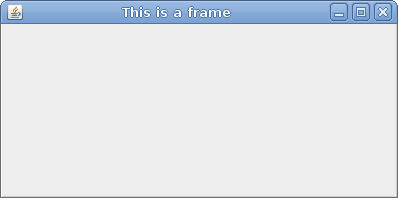
\includegraphics[width=0.6\linewidth]{frame}
\end{center}
\end{frame}

\section{Components}
\subsection{Adding components}
\begin{frame}[fragile]
  \frametitle{Adding components to our frame}
  \begin{verbatim}
public static void main(String[] args) {
  JFrame frame = new JFrame("This is a frame");
  frame.setPreferredSize(new Dimension(400, 200));
  frame.setDefaultCloseOperation(JFrame.EXIT_ON_CLOSE);

  JPanel panel = new JPanel();
  frame.setContentPane(panel);
  panel.add(new JLabel("Hello World!"));

  frame.pack();
  rframe.setVisible();
}
\end{verbatim}
\begin{center}
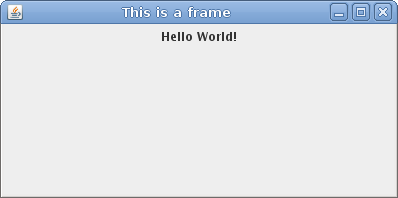
\includegraphics[width=0.6\linewidth]{label}
\end{center}
\end{frame}

\tikzstyle{level 1}=[level distance=3cm, sibling distance=1cm]
\tikzstyle{level 2}=[level distance=4cm, sibling distance=1.5cm]
\tikzstyle{level 3}=[level distance=3cm, sibling distance=1cm]

\subsection{Components Hierarchy}
\begin{frame}[fragile, shrink]
  \frametitle{Components Hierarchy}
\begin{center}
\begin{tikzpicture}[grow=right]
  \node {\verb!JComponent!}
  child {
    node {\verb!JTextComponent!}
    child{
      node {\verb!JTextArea!}
    }
    child{
      node {\verb!JEditorPane!}
      child{
        node{\verb!JTextPane!}
      }
    }
    child{
      node {\verb!JTextField!}
      child{
        node{\verb!JPasswordField!}
      }
    }
  }
  child{
    node {\verb!JComboBox!}
  }
  child{
    node {\verb!JLabel!}
  }
  child{
    node {\verb!JList!}
  }
  child{
    node {\verb!JMenuBar!}
  }
  child{
    node {\verb!JPanel!}
  }
  child{
    node {\verb!JPopupMenu!}
  }
  child{
    node {\verb!JScrollBar!}
  }
  child{
    node {\verb!JScrollPane!}
  }
  child {
    node {\verb!AbstractButton!}
    child {
      node {\verb!JToggleButton!}
      child{
        node {\verb!JCheckBox!}
      }
      child{
        node{\verb!JRadioButton!}
      }
    }
    child {
      node {\verb!JButton!}
    }
    child {
      node {\verb!JMenuItem!}
      child {
        node {\verb!JCheckBoxMenuItem!}
      }
      child {
        node {\verb!JMenu!}
      }
      child {
        node {\verb!JRadioButtonMenuItem!}
      }
    }
  };
\end{tikzpicture}
\end{center}
\end{frame}

\section{Layouts}
\begin{frame}[fragile]
  \frametitle{JPanel and layouts}
  \begin{itemize}
    \item \verb!JPanel! are containers that group and arrange other components.
    \item We add a component to a \verb!JPanel! with the \verb!.add(component)! method.
    \item Components inside a \verb!JPanel! are placed according to its
      \alert{layout}.
    \item Layouts implement the API interface \verb!LayoutManager!.
    \item We choose a JPanel's layout in its constructor \verb! new JPanel(new FlowLayoutDemo())!.
  \end{itemize}
\begin{center}
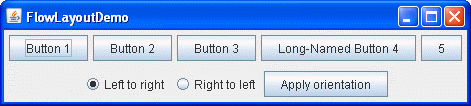
\includegraphics[width=0.6\linewidth]{FlowLayoutDemo1}
\end{center}
\end{frame}

\begin{frame}[fragile]
  \frametitle{Some examples of layouts}
  \begin{center}
    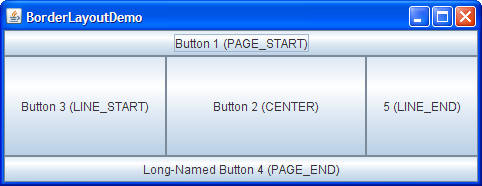
\includegraphics[width=0.6\linewidth]{BorderLayoutDemo}
  \end{center}
  \begin{center}
    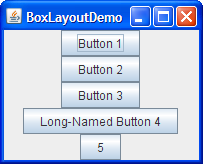
\includegraphics[width=0.4\linewidth]{BoxLayoutDemo}
  \end{center}
\end{frame}

\begin{frame}[fragile]
  \frametitle{More complex layouts}
  \begin{itemize}
    \item There are more complex layouts available, see:
      \verb!http://java.sun.com/docs/books/tutorial/uiswing/layout/!
    \item Using hierarchies of layouts, you can place your components very precisely.
  \end{itemize}
\end{frame}

\section{Event listeners}

\subsection{Clicking on a button}
\begin{frame}[fragile]
  \frametitle{Clicking on a button}
\begin{verbatim}
JButton button = new JButton("Hello!");
panel.add(button);
\end{verbatim}
\begin{center}
  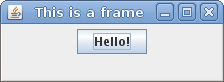
\includegraphics[width=0.38\linewidth]{beforeClick}
  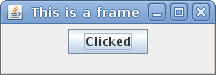
\includegraphics[width=0.4\linewidth]{afterClick}
\end{center}
\structure{How to react to an action from the user ?}
\end{frame}

\subsection{Listeners}
\begin{frame}[fragile]
  \frametitle{Listener interface}
\begin{verbatim}
import java.awt.event.*;
class ButtonListener implements ActionListener {
  JButton button;
  public ButtonListener(JButton button){
    this.button = button;
  }
  public void actionPerformed(ActionEvent e) {
    button.setLabel("Clicked");
  }
}

button.addActionListener(new ButtonListener(button));
\end{verbatim}
\end{frame}

\begin{frame}[fragile]
  \frametitle{Anonymous classes and listeners}
\begin{verbatim}
button.addActionListener(
  new ActionListener() {
    public void actionPerformed(ActionEvent e) {
      button.setLabel("Clicked");
    }
  });
\end{verbatim}
\end{frame}

\begin{frame}
  \frametitle{More on listeners}
  \begin{itemize}
    \item More details on listeners at:
      \verb!http://java.sun.com/docs/books/tutorial/uiswing/events/!
  \end{itemize}
\end{frame}

\section{Drawing}
\begin{frame}
  \frametitle{Drawing}
  \begin{itemize}
    \item Override the JComponent's method \verb!void paintComponent(Graphics g)!.
    \item This method is called each time the component must be redrawn.
    \item The \verb!Graphics! object lets you draw inside the Component.
    \item For a JFrame you can override the paint method.
    \item See example!
  \end{itemize}
\end{frame}

\section{Making your own components}
\begin{frame}
  \frametitle{Making your own components}
  \begin{itemize}
    \item As any other java class, \verb!JComponent! can be extended.
    \item This can be useful in many cases:
      \begin{itemize}
        \item Factorizing a component and its listeners in the same class.
        \item Changing the look of a component.
        \item Adding functionalities to a component.
      \end{itemize}
  \end{itemize}
\end{frame}

\end{document}
